\clearpage
\section{Zweitore, Vierpole}
\subsection{Zweitorgleichungen}
\renewcommand{\arraystretch}{1.2}
%\small
% \includegraphics[width=\columnwidth]{Zweipole/Zweitorgleichungen}
    \begin{itemize}[leftmargin=*]
        \item{Admittanzform/ Admittanzmatrix \textbf{Y}:}
        \begin{align*}
            \begin{split}
                \underline{I}_1 &= \underline{Y}_{11}\cdot\underline{U}_1 + \underline{Y}_{12}\cdot\underline{U}_2\\
                \underline{I}_2 &= \underline{Y}_{21}\cdot\underline{U}_1 + \underline{Y}_{22}\cdot\underline{U}_2
            \end{split} \qquad
            {\begin{pmatrix}
                \underline{I}_1 \\
                \underline{I}_2
            \end{pmatrix}} = \textbf{\underline{Y}}\cdot
            \begin{pmatrix}
                \underline{U}_1 \\
                \underline{U}_2
            \end{pmatrix}      
        \end{align*}
        \item{Impedanzform/ Impedanzmatrix \textbf{Z}:}
            \begin{align*}
                \begin{split}
                \underline{U}_1 &=\underline{Z}_{11}\cdot\underline{I}_1 + \underline{Z}_{12}\cdot\underline{I}_2 \\
                \underline{U_2} &=\underline{Z}_{21}\cdot\underline{I}_1 + \underline{Z}_{22}\cdot\underline{I}_2
                \end{split}\qquad
                \begin{pmatrix}
                    \underline{U}_1 \\
                    \underline{U}_2
                \end{pmatrix} = \textbf{\underline{Z}}\cdot
                \begin{pmatrix}
                    \underline{I}_1 \\
                    \underline{I}_2
                \end{pmatrix}  
            \end{align*}
        \item{Hybridform 1/ Reihenparallelmatrix \textbf{H}:}
            \begin{align*}
                \begin{split}
                    \underline{U}_1 &= \underline{H}_{11}\cdot\underline{I}_1 + \underline{H}_{12}\cdot\underline{U}_2 \\
                    \underline{I}_2 &= \underline{H}_{21}\cdot\underline{I}_1 + \underline{H}_{22}\cdot\underline{U}_2
                \end{split}
				\qquad	
                \begin{pmatrix}
                    \underline{U}_1 \\
                    \underline{I}_2
                \end{pmatrix} = \textbf{\underline{H}}\cdot
                \begin{pmatrix}
                    \underline{I}_1 \\
                    \underline{U}_2
                \end{pmatrix}
            \end{align*}
            \item{Hybridform 2/ Parallelreihenmatrix \textbf{C}:}
            \begin{align*}
                \begin{split}
                    \underline{I}_1 &= \underline{C}_{11}\cdot\underline{U}_1 + \underline{C}_{12}\cdot\underline{I}_2 \\
                    \underline{U}_2 &= \underline{C}_{21}\cdot\underline{U}_1 + \underline{C}_{22}\cdot\underline{I}_2
                \end{split}
				\qquad
                \begin{pmatrix}
                    \underline{I}_1 \\
                    \underline{U}_2
                \end{pmatrix} = \textbf{\underline{C}}\cdot
                \begin{pmatrix}
                    \underline{U}_1 \\
                    \underline{I}_2
                \end{pmatrix}
            \end{align*}
            
            \item{Kettenform/ Kettenmatrix \textbf{A}:}
                \begin{align*}
                    \begin{split}
                        \underline{U}_1 &= \underline{A}_{11}\cdot\underline{U}_2 + \underline{A}_{12}\cdot-\underline{I}_2 \\
                        \underline{I}_1 &= \underline{A}_{21}\cdot\underline{U}_2 + \underline{A}_{22}\cdot-\underline{I}_2
                    \end{split}
	               \qquad
                    \begin{pmatrix}
                        \underline{U}_1 \\
                        \underline{I}_2
                    \end{pmatrix} = \textbf{\underline{A}}\cdot
                    \begin{pmatrix}
                        \underline{U}_2 \\
                        -\underline{I}_2
                    \end{pmatrix}
                \end{align*}
%                \item{Kettenform rückwärts/ Kettenmatrix \textbf{B}:}
%                    \begin{align*}
%                        \begin{split}
%                            \underline{U}_2 &= \underline{B}_{11}\cdot\underline{U}_1 + \underline{B}_{12}\cdot-\underline{I}_1\\
%                            \underline{I}_2 &= \underline{B}_{21}\cdot\underline{U}_1 + \underline{B}_{22}\cdot-\underline{I}_1
%                        \end{split}
%                    \qquad
%                    \begin{pmatrix}
%                        \underline{U}_2\\
%                        \underline{I}_2
%                    \end{pmatrix} = \textbf{\underline{B}}\cdot
%                    \begin{pmatrix}
%                        \underline{U}_1 \\
%                        -\underline{I}_1
%                    \end{pmatrix}
%                    \end{align*}
    \end{itemize}
   \normalsize
   
\subsubsection{Matrizenrechnung}
siehe Papula FS S.204f.
\[  [\operatorname{\underline{A}}]\cdot [\operatorname{\underline{B}}] = [\underline{C}] \rightarrow  \begin{bmatrix}
	a_{11} & a_{12}\\ 
	a_{21} & a_{22} 
\end{bmatrix}
\cdot
\begin{bmatrix}
	b_{11} & b_{12}\\ 
	b_{21} & b_{22}  
\end{bmatrix}
=
\begin{bmatrix}
	c_{11} & c_{12}\\ 
	c_{21} & c_{22}   
\end{bmatrix} \] 
Bsp.: $c_{21}=a_{21}\cdot b_{11} + a_{22} \cdot b_{21}$
\[ \det(A)=a_{11}\cdot a_{22} - a_{12} \cdot a_{21} \] 
$\det(A)=0 \rightarrow$ nicht inventierbar.
\subsubsection{Parameterumrechnung}
{ \renewcommand{\arraystretch}{1.6}
	\arraycolsep=1.3pt
\begin{tabular}{|c|c|c|c|c|c|}
	\hline
	 & geg. \underline{$\mathbf{A}$}& geg. \underline{$\mathbf{Z}$} & geg. \underline{$\mathbf{Y}$} & geg. \underline{$\mathbf{H}$} & geg. \underline{$\mathbf{C}$}\\
	\hline
	\makecell{ges. \\ \underline{$\mathbf{A}$}}& $\begin{matrix}
		\underline{A}_{11} & \underline{A}_{12} \\
		\underline{A}_{21} & \underline{A}_{22}
	\end{matrix}$ & $\begin{matrix}
		\frac{Z_{11}}{Z_{21}} & \frac{\det Z}{Z_{21}} \\
		\frac{1}{Z_{21}} & \frac{Z_{22}}{Z_{21}}
	\end{matrix}$ & $\begin{matrix}
	\frac{-Y_{22}}{Y_{21}} & \frac{-1}{Y_{21}} \\
	\frac{-\det Y}{Y_{21}} & \frac{-Y_{11}}{Y_{21}}
	\end{matrix}$ & $\begin{matrix}
	\frac{-\det H}{H_{21}} & \frac{-H_{11}}{H_{21}} \\
	\frac{-H_{22}}{H_{21}} & \frac{-1}{H_{21}}
	\end{matrix}$ & $\begin{matrix}
	\frac{1}{C_{21}} & \frac{C_{22}}{C_{21}} \\
	\frac{C_{11}}{C_{21}} & \frac{\det C}{C_{21}}
	\end{matrix}$\\
	\hline
	\makecell{ges. \\ \underline{$\mathbf{Z}$}}& $\begin{matrix}
		\frac{A_{11}}{A_{21}} & \frac{\det A}{Z_{21}} \\
		\frac{1}{A_{21}} & \frac{A_{22}}{A_{21}}
	\end{matrix}$ & $\begin{matrix}
		\underline{Z}_{11} & \underline{Z}_{12} \\
		\underline{Z}_{21} & \underline{Z}_{22}
	\end{matrix}$ & $\begin{matrix}
	\frac{Y_{22}}{\det Y} & \frac{-Y_{12}}{\det Y} \\
	\frac{-Y_{21}}{\det Y} & \frac{Y_{11}}{\det Y}
	\end{matrix}$ & $\begin{matrix}
	\frac{\det H}{H_{22}} & \frac{H_{12}}{H_{22}} \\
	\frac{-H_{21}}{H_{22}} & \frac{1}{H_{22}}
	\end{matrix}$ & $\begin{matrix}
	\frac{1}{C_{11}} & \frac{-C_{12}}{C_{11}} \\
	\frac{C_{21}}{C_{11}} & \frac{\det C}{C_{11}}
	\end{matrix}$\\
	\hline
	\makecell{ges. \\ \underline{$\mathbf{Y}$}}& $\begin{matrix}
		\frac{A_{22}}{A_{12}} & \frac{-\det A}{A_{12}} \\
		\frac{-1}{A_{12}} & \frac{A_{11}}{A_{12}}
	\end{matrix}$ & $\begin{matrix}
	\frac{Z_{22}}{\det Z} & \frac{-Z_{12}}{\det Z} \\
	\frac{-Z_{21}}{\det Z} & \frac{Z_{11}}{\det Z}
	\end{matrix}$  & $\begin{matrix}
	\underline{Y}_{11} & \underline{Y}_{12} \\
	\underline{Y}_{21} & \underline{Y}_{22}
	\end{matrix}$ & $\begin{matrix}
	\frac{1}{H_{11}} & \frac{-H_{12}}{H_{11}} \\
	\frac{H_{21}}{H_{11}} & \frac{\det H}{H_{11}}
	\end{matrix}$   & $\begin{matrix}
	\frac{\det C}{C_{22}} & \frac{C_{12}}{C_{22}} \\
	\frac{-C_{21}}{C_{22}} & \frac{1}{C_{22}}
	\end{matrix}$\\
	\hline
	\makecell{ges. \\ \underline{$\mathbf{H}$}} & $\begin{matrix}
		\frac{A_{12}}{A_{22}} & \frac{\det A}{A_{22}} \\
		\frac{-1}{A_{22}} & \frac{A_{21}}{A_{22}}
	\end{matrix}$ & $\begin{matrix}
	\frac{\det Z}{Z_{22}} & \frac{Z_{12}}{Z_{22}} \\
	\frac{-Z_{21}}{Z_{22}} & \frac{1}{Z_{22}}
	\end{matrix}$ & $\begin{matrix}
	\frac{1}{Y_{11}} & \frac{-Y_{12}}{Y_{11}} \\
	\frac{Y_{21}}{Y_{11}} & \frac{\det Y}{Y_{11}}
	\end{matrix}$ & $\begin{matrix}
		\underline{H}_{11} & \underline{H}_{12} \\
		\underline{H}_{21} & \underline{H}_{22}
	\end{matrix}$& $\begin{matrix}
	\frac{C_{22}}{\det C} & \frac{-C_{12}}{\det C} \\
	\frac{-C_{21}}{\det C} & \frac{C_{11}}{\det C}
	\end{matrix}$\\
	\hline
	\makecell{ges. \\ \underline{$\mathbf{C}$}}& $\begin{matrix}
		\frac{A_{21}}{A_{11}} & \frac{-\det A}{A_{11}} \\
		\frac{-1}{A_{11}} & \frac{A_{12}}{A_{11}}
	\end{matrix}$ & $\begin{matrix}
	\frac{1}{Z_{11}} & \frac{-Z_{12}}{Z_{11}} \\
	\frac{Z_{21}}{Z_{11}} & \frac{\det Z}{Z_{11}}
	\end{matrix}$ & $\begin{matrix}
	\frac{\det Y}{Y_{22}} & \frac{Y_{12}}{Y_{22}} \\
	\frac{-Y_{21}}{Y_{22}} & \frac{1}{Y_{22}}
	\end{matrix}$ & $\begin{matrix}
	\frac{H_{22}}{\det H} & \frac{-H_{12}}{\det H} \\
	\frac{-H_{21}}{\det H} & \frac{H_{11}}{\det H}
	\end{matrix}$ & $\begin{matrix}
	\underline{C}_{11} & \underline{C}_{12} \\
	\underline{C}_{21} & \underline{C}_{22}
	\end{matrix}$ \\
	\hline
\end{tabular} }

\subsection{Betriebsarten, Bezugspfeilsystem}
\begin{minipage}{0.5\columnwidth}
	\small
	Betrieb von Seite 1,\\ Last an Tor 2.\\
	
	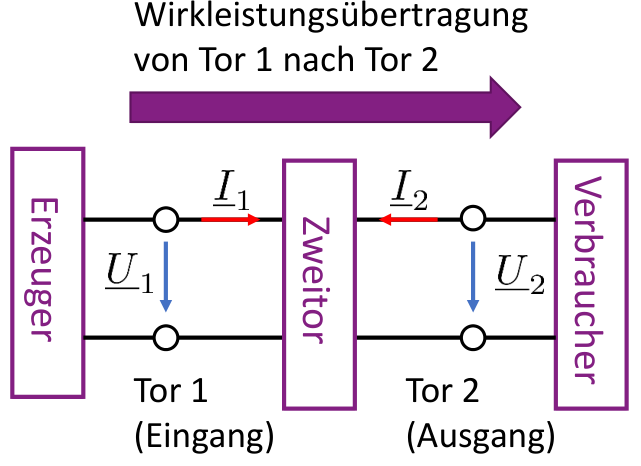
\includegraphics[width=\columnwidth]{Zweipole/betrieb_seite_1}
\end{minipage}
%\vspace{1em}
\begin{minipage}{0.5\columnwidth}
	\small
	Betrieb von Seite 2,\\ Last an Tor 1.\\
	
	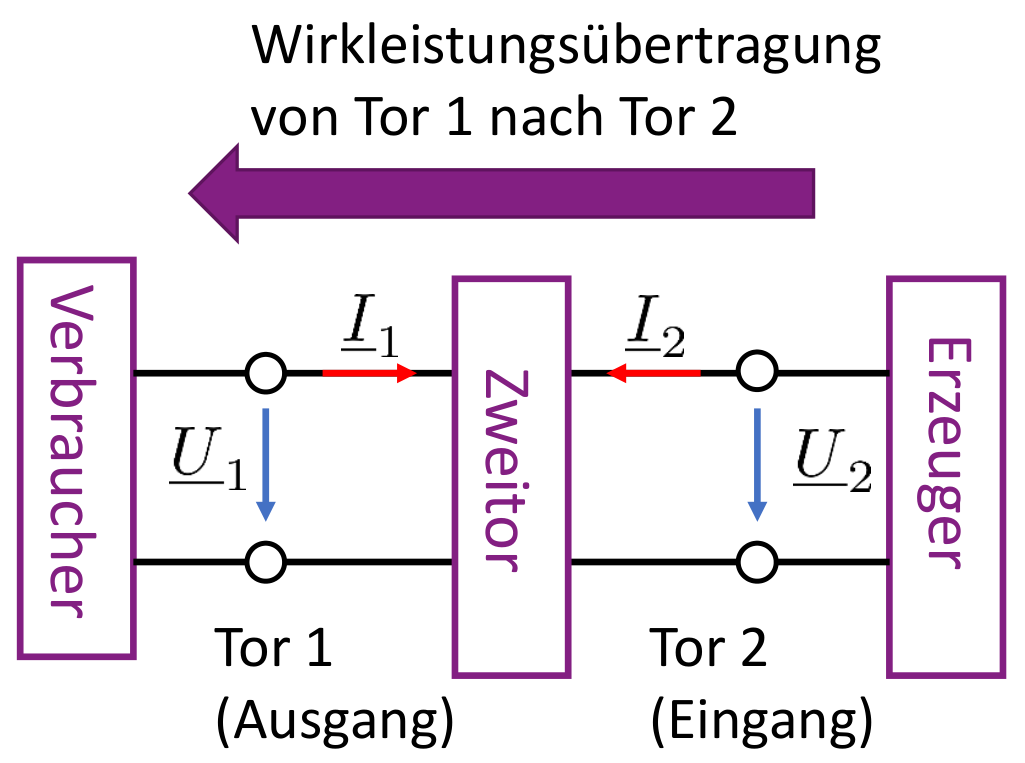
\includegraphics[width=\columnwidth]{Zweipole/betrieb_seite_2}
\end{minipage}\\
\setlength{\parindent}{0pt}\\
Bild zeigt: Symmetrisches Bezugspfeilsystem.
\subsection{ZT-Eigenschaften}
\small
\begin{tabularx}{0.85\columnwidth}{|c|c|c|X|}
	\hline
	& Umkehrbarkeit & Symmetrie & Rückwirkungs-freiheit\\
	\hline\hline
	$Z$&  $Z_{12} = Z_{21}$ & $Z_{11} = Z_{22}$ & $Z_{12} = 0$\\
	\hline
	$Y$&  $Y_{12} = Y_{21}$& $Y_{11} = Y_{22}$ & $Y_{12 } = 0$ \\
	\hline
	$A$&  $\operatorname{det}[A] = 1$& $A_{11} = A_{22}$ & $\operatorname{det}[A] = 0$\\
	\hline
	$H$&  $H_{12} = -H_{21}$& $\operatorname{det}[H]=1$ & $H_{12} = 0$ \\
	\hline
	$C$&  $C_{12} = -C_{21}$& $\operatorname{det}[C]=1$ & $C_{12} = 0$ \\
		\hline
\end{tabularx}\\
\begin{itemize}[leftmargin=*]
	\item Umkehrbares (reziprokes) ZT: nur 3 Parameter, Ursache und Wirkung tauschen Torseiten $\rightarrow$ gleiches Verhalten.
	\item (Widerstands-)symmetrisches ZT: Eingangswiderstände in beiden Betriebsarten gleich, Ein- und Ausgang vertauschbar.
	\item Umkehrbares und symmetrisches ZT = längssymmetrisch: nur 2 Parameter.
	\item Passives ZT aus R,L,C,M-Bauteilen ist immer umkehrbar.
	\item Rückwirkungsfreies (unilaterales) ZT: nur 3 Parameter, Energieübertragung nur von Eingang auf Ausgang.
\end{itemize}
\clearpage
\begin{samepage}
    \subsection{Matrizen elementarer Zweitore}
    \begin{center}
    	\includegraphics[width=\textwidth]{Zweipole/Tabellen und Ergänzungen_Zweitormatrizen}
    \end{center}
\end{samepage}
\clearpage

\subsection{Zusammenschalten von Zweitoren}
\subsubsection{Torbedingungen}
\small
Erfüllung durch: ideale \"Ubertrager, Kurzschlussschleife, Parallelschaltung längs-symmetrischer Zweitore.
\normalsize
\subsubsection{Zweitor-Schaltungen}
Torbedingung muss für ZT-Schaltungen erfüllt sein!\\

\begin{minipage}{0.45\columnwidth}
		\centering Reihenschaltung
	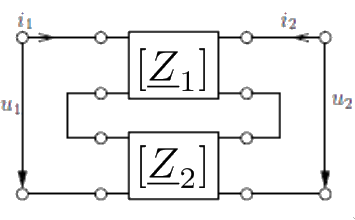
\includegraphics[width=0.8\columnwidth]{Zweipole/Reihenschaltung_Zweitore}
	\[
	\left[ \underline{Z} \right] = \left[ \underline{Z}_1 \right] + \left[ \underline{Z}_2 \right]
	\]
\end{minipage}
\begin{minipage}{0.45\columnwidth}
	\centering Parallelschaltung
	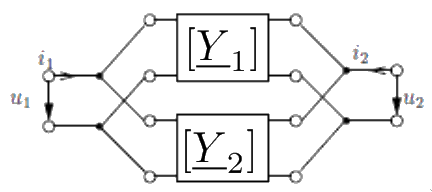
\includegraphics[width=\columnwidth]{Zweipole/Parallelschaltung_Zweitoren}
	\[
	\left[ \underline{Y} \right] = \left[ \underline{Y}_1 \right] + \left[ \underline{Y}_2 \right]
	\]
\end{minipage}  \\

\begin{minipage}{0.45\columnwidth}
			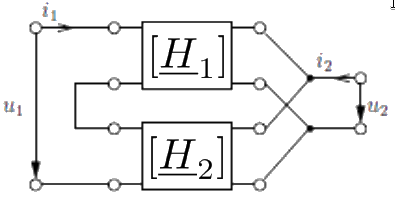
\includegraphics[width=\columnwidth]{Zweipole/Reihen-Parallelschaltung_Zweitoren}
			 Reihen-Parallelschaltung
	\[
	\left[ \underline{H} \right] = \left[ \underline{H}_1 \right] \cdot \left[ \underline{H}_2 \right]
	\]
\end{minipage}
\begin{minipage}{0.45\columnwidth}
			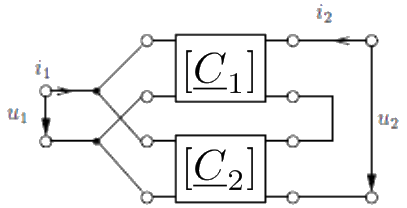
\includegraphics[width=\columnwidth]{Zweipole/Parallel-Reihenschaltung_Zweitoren}
			Parallel-Reihenschaltung
	\[
	\left[ \underline{C} \right] = \left[ \underline{C}_1 \right] \cdot \left[ \underline{C}_2 \right]
	\]
\end{minipage}

\begin{itemize}
	\item \textbf{Kettenschaltung}:\\
	Torbedingung wird immer eingehalten!
	\begin{center}
		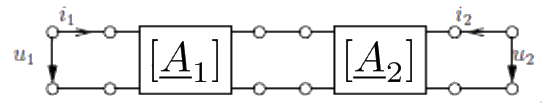
\includegraphics[width=0.6\columnwidth]{Zweipole/Kettenschaltung_Zweitoren}
		\[
		\left[ \underline{A} \right] = \left[ \underline{A}_1 \right] \cdot \left[ \underline{A}_2 \right] \neq \left[ \underline{A}_2
		\right] \cdot \left[ \underline{A}_1 \right]
		\]
	\end{center}
	\normalsize Reihenfolge beachten! \textbf{Nicht} kommutativ!
\end{itemize}
\subsubsection{Idealer Trennverst\"arker/OP} \label{trennverstärker}
Idealer Trennverstärker  $\text{v}_U$ als idealer OP.\\ 
Zweck: Rückwirkungsfreiheit einer Kettenschaltung.\\
Entspricht einer VCVS.\\
\begin{minipage}{0.5\columnwidth}
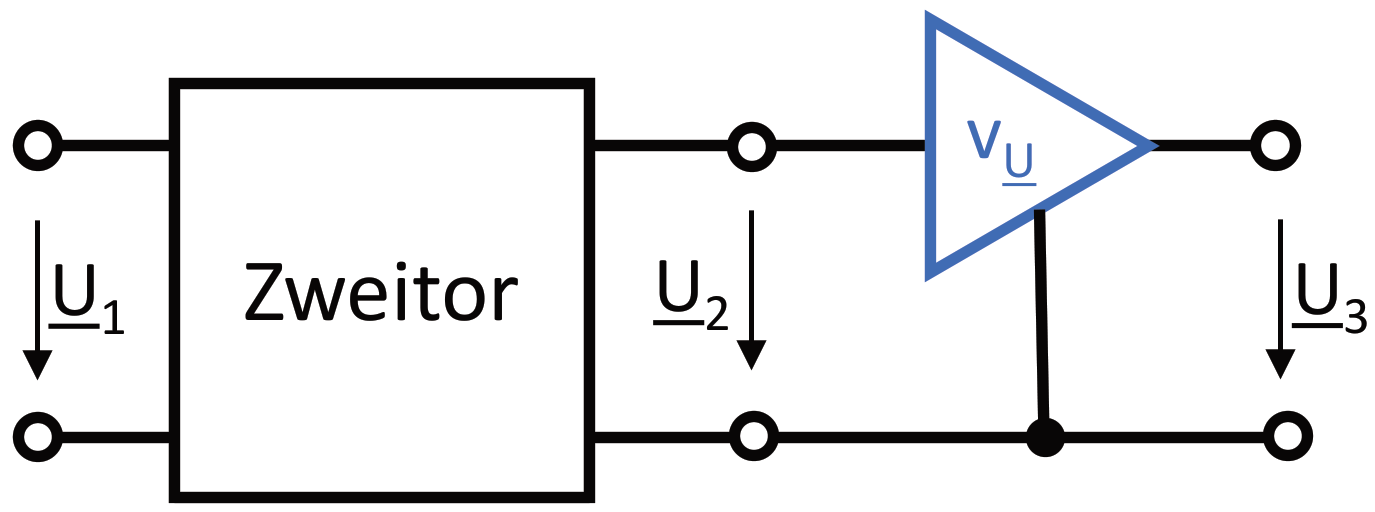
\includegraphics[width=1.2\columnwidth]{Zweipole/Trennverstaerker}
\end{minipage}
\begin{minipage}{0.5\columnwidth}
	\renewcommand*{\arraystretch}{1.7}
	\[
	[\underline{A}] = \begin{pmatrix}
		\dfrac{1}{\text{v}_U} & 0 \\
		0        & 0
	\end{pmatrix}
	\]
\end{minipage}

\begin{equation*}
	\boxed{
	\underline{Z}_E \rightarrow \infty \quad \underline{Z}_A = 0 \quad \underline{\text{v}}_{\text{D}}\rightarrow \infty \quad \text{v}_U = \text{konst.}}
\end{equation*}
{\small
	$Z_{E/A}$: Ein-/Ausgangswiderstand, $v_D$: Differenzverstärkung.
}
\subsubsection{Operationsverstärker (OP)}
\begin{itemize}[leftmargin=*]
	\item nicht-inventierender OP\\
			\begin{minipage}{0.4\columnwidth}
				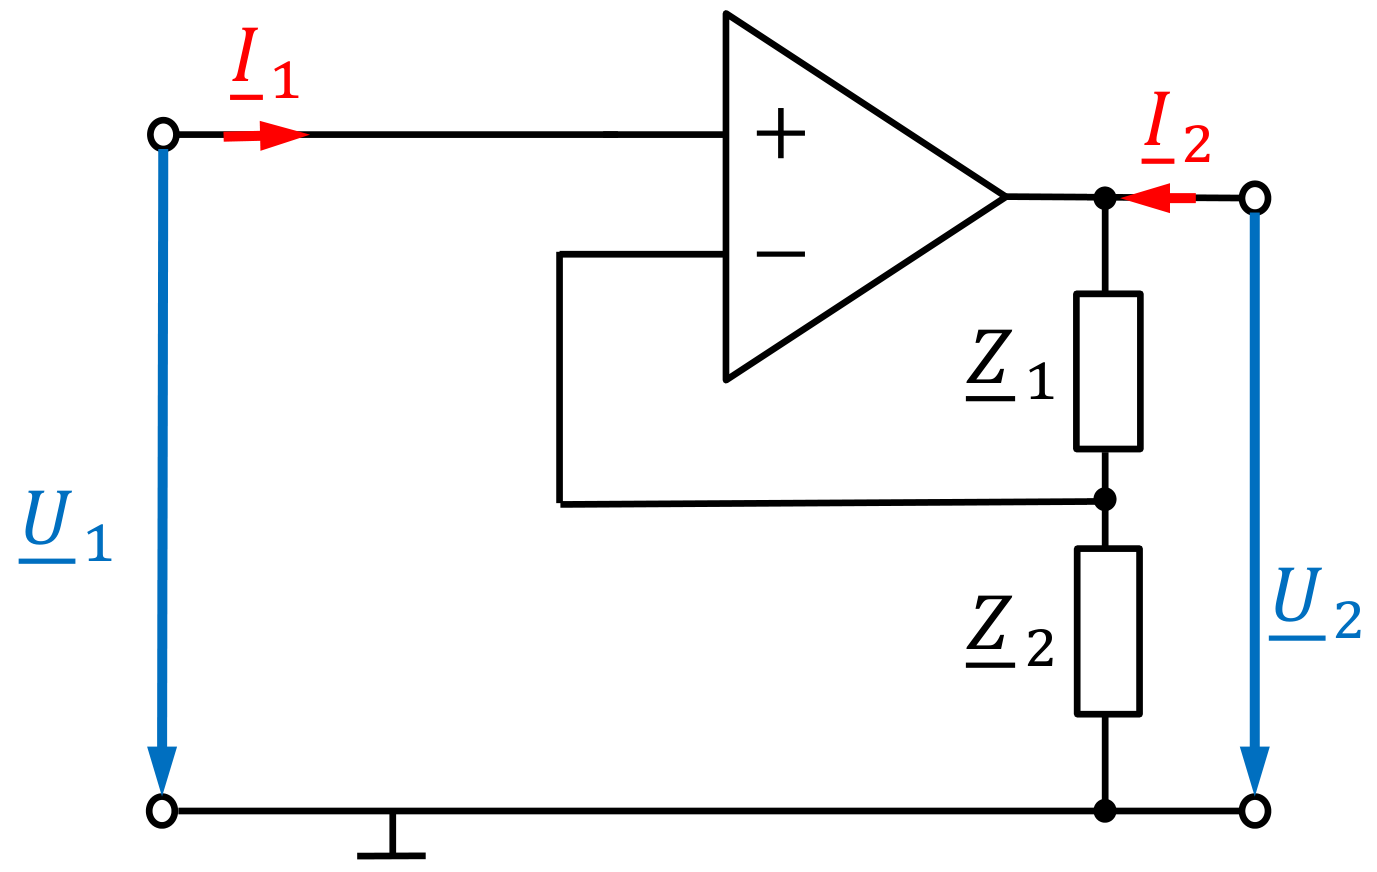
\includegraphics[width=\columnwidth]{Zweipole/nichtinventierender_op}
			\end{minipage}
			\begin{minipage}{0.6\columnwidth}
				\renewcommand*{\arraystretch}{1.7}
				\begin{equation*}
					[\underline{A}] = \begin{pmatrix}
						\frac{1}{\nu_D} + \frac{\underline{Z}_2}{\underline{Z}_1 + \underline{Z}_2} & \frac{\underline{Z}_A}{\nu_D} \\
						\frac{1}{\nu_D \underline{Z}_E} & \frac{\underline{Z}_A}{\nu_D \underline{Z}_E}
					\end{pmatrix}
				\end{equation*}
			Für idealen OP $\rightarrow$ \\
			$Z_E\rightarrow\infty, Z_A=0, v_D\rightarrow\infty$.
			\vspace{1.1em}
			\end{minipage}
			ideale Spannungs-Verstärkung:
			\begin{equation*}
				\text{v}_u=\frac{\underline{U}_2}{\underline{U}_1}=
				\frac{1}{\underline{A}_{11}}=\frac{\underline{Z}_1+\underline{Z}_2}{\underline{Z}_2} = 1 + \frac{\underline{Z}_1}{\underline{Z}_2}
			\end{equation*}
	\item inventierender OP\\
	\begin{minipage}{0.4\columnwidth}
		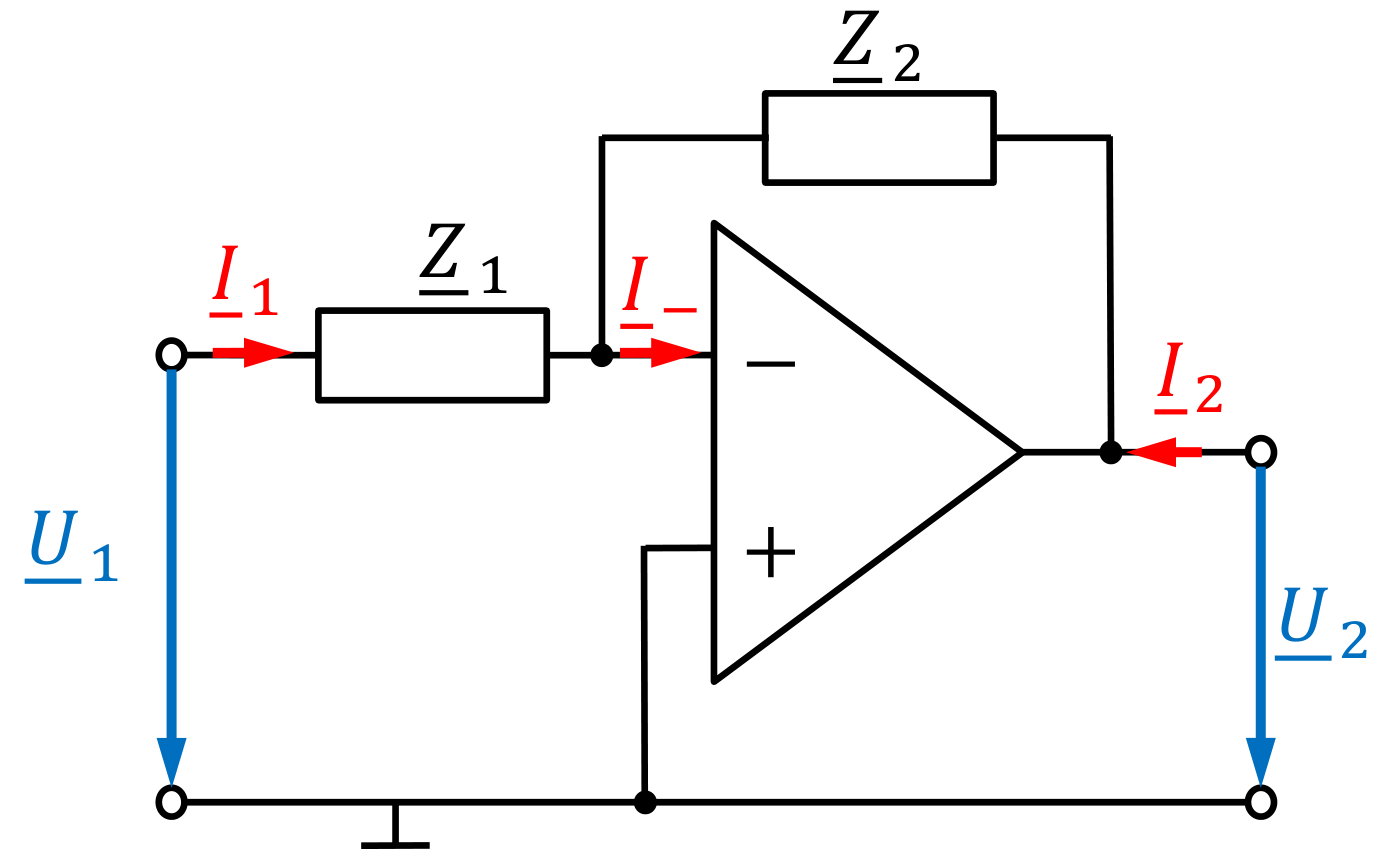
\includegraphics[width=\columnwidth]{Zweipole/inventierender_op}
	\end{minipage}
	\begin{minipage}{0.6\columnwidth}
		\renewcommand*{\arraystretch}{1.7}
		Allgemein, für idealen OP $\rightarrow$ \\
		$Z_E\rightarrow\infty,\, Z_A=0,\, v_D\rightarrow\infty$.
		\begin{equation*}
			[\underline{A}] \approx - \begin{pmatrix}
				\frac{\underline{Z}_1}{\underline{Z}_2} & 0 \\
				\frac{1}{\underline{Z}_2} & 0
			\end{pmatrix}
		\end{equation*}
			\vspace{1em}
	\end{minipage}
			ideale Spannungs-Verstärkung:
	\begin{equation*}
		\text{v}_u=\frac{1}{\underline{A}_{11}}=\frac{\underline{U}_2}{\underline{U}_1}=-\frac{\underline{Z}_2}{\underline{Z}_1}
	\end{equation*}
\end{itemize}

\subsection{Ersatzschaltbilder}
\subsubsection{Ideale gesteuerte Quellen}
Ideale gesteuerte Quellen \textbf{nicht} ineinander umwandelbar!\\
\begin{minipage}[t]{0.5\columnwidth}
\footnotesize
VCVS: Spannungsgesteuerte\\ Spannungsquelle
\normalsize
\begin{center}
	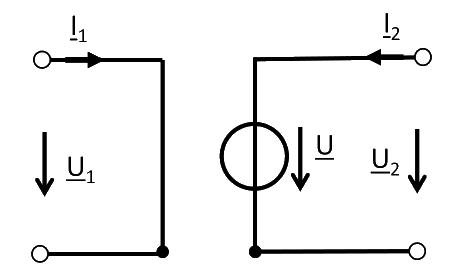
\includegraphics[width=0.9\columnwidth]{Zweipole/spg-spg-gestuert}\\
	\begin{tabular}{cc}
		VCVS:& $\underline{U}=\alpha\cdot \underline{U}_1$
	\end{tabular}
\end{center}
\end{minipage}
\vspace{1em}
\begin{minipage}[t]{0.5\columnwidth}
 \footnotesize
	CCVS: Stromgesteuerte \\ Spannungsquelle
	\normalsize
	\vspace{-0.4em}
	\begin{center}
		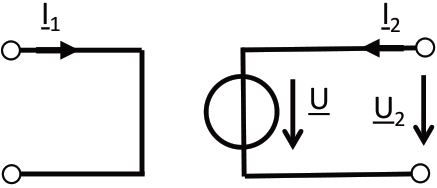
\includegraphics[width=0.9\columnwidth]{Zweipole/strm-spg-gestuert}\\
		\begin{tabular}{cc}
				CCVS: & $\underline{U}=\underline{Z}_T\cdot \underline{I}_1$
		\end{tabular}
	\end{center}
\end{minipage}
\\
\begin{minipage}[t]{0.5\columnwidth}
	\footnotesize
	VCCS: Spannungsgesteuerte\\ Stromquelle
	\normalsize
	\begin{center}
		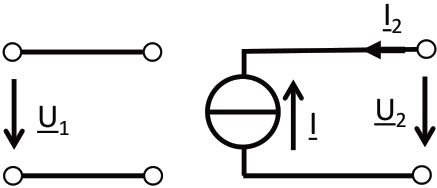
\includegraphics[width=0.9\columnwidth]{Zweipole/spg-strm-gestuert}\\
		\begin{tabular}{cc}
			VCCS:& $\underline{I}=\underline{Y}_T\cdot \underline{U}_1$
		\end{tabular}
	\end{center}
\end{minipage}
\begin{minipage}[t]{0.5\columnwidth}
	\footnotesize
	CCCS: Stromgesteuerte\\ Stromquelle
	\normalsize
	\begin{center}
		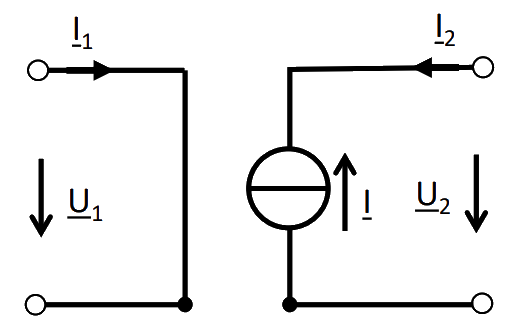
\includegraphics[width=0.9\columnwidth]{Zweipole/strm-strm-gesteuert}\\
		\begin{tabular}{cc}
			CCCS:& $\underline{I}=\beta\cdot \underline{I}_1$
		\end{tabular}
	\end{center}
\end{minipage}
 \vspace{1em}

{	\renewcommand{\arraystretch}{1.2}
	\arraycolsep=1.3pt
\begin{tabular}{|c|c|c|c|c|}
	\hline
	& VCVS& VCCS & CCVS & CCCS\\
	\hline
	[\underline{A}]& $\begin{matrix}
		\alpha^{-1} & 0 \\
		0 & 0
	\end{matrix}$ & $\begin{matrix}
		0 & -\underline{Y}_T^{-1} \\
		0 & 0
	\end{matrix}$ & $\begin{matrix}
	0 & 0 \\
\underline{Z}_T^{-1} & 0
	\end{matrix}$ & $\begin{matrix}
	0 & 0 \\
	0 & -\beta^{-1}
	\end{matrix}$\\
	\hline
	[\underline{Z}]& & & $\begin{matrix}
		\underline{Z}_T & 0 \\
		0 & 0
	\end{matrix}$ &\\
	\hline
	[\underline{Y}]& & $\begin{matrix}
		0 & 0 \\
		-\underline{Y}_T & 0
	\end{matrix}$ & & \\
	\hline
	[\underline{H]}& & & & $\begin{matrix}
		0 & 0 \\
		-\beta & 0
	\end{matrix}$\\
	\hline
	[\underline{C}]& $\begin{matrix}
		0 & 0 \\
		\alpha & 0
	\end{matrix}$ & & &\\
	\hline
\end{tabular} }
\subsubsection{Lineare gesteuerte Quellen}
Alle Darstellungen sind äquivalent und lassen sich ineinander umwandeln!\\
    \begin{minipage}{0.5\columnwidth}
    	\renewcommand{\arraystretch}{1.3}
        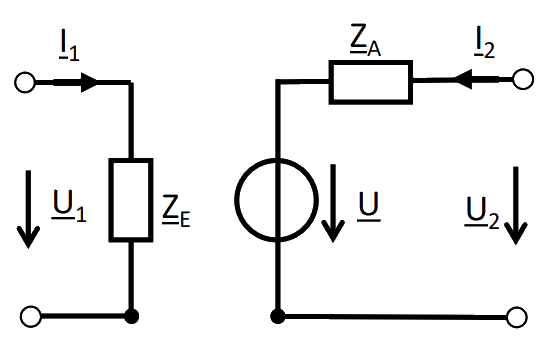
\includegraphics[width=0.9\columnwidth]{Zweipole/spg-spg-gestuert_linear}\\
    \begin{tabular}{ll}
        VCVS:& $\underline{U}=\alpha\cdot \underline{U}_1$\\
        VCCS:& $\underline{I}=\underline{Y}_T\cdot \underline{U}_1$
    \end{tabular}
    \end{minipage}
    \begin{minipage}{0.5\columnwidth}
    	\renewcommand{\arraystretch}{1.3}
        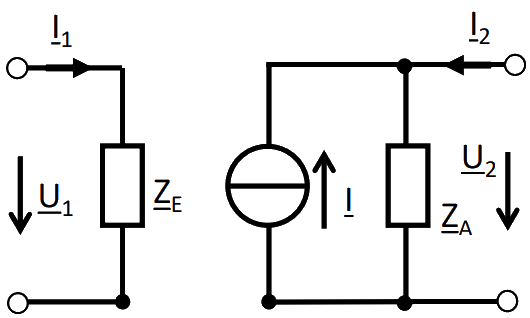
\includegraphics[width=0.9\columnwidth]{Zweipole/strm-strm-gesteuert_linear}\\
    \begin{tabular}{ll}
    	        CCVS:& $\underline{U}=\underline{Z}_T\cdot \underline{I}_1 $\\
        CCCS:& $\underline{I}=\beta\cdot \underline{I}_1$
    \end{tabular}
    \end{minipage}

\subsubsection{Ersatzschaltbilder (ESB)}
\begin{itemize}
    \item \textbf{T-ESB} bei gegebener $[\underline{Z}]$-Matrix:
   
    	$Z_{12} \neq Z_{21}$ mit gesteuerter Quelle. 
        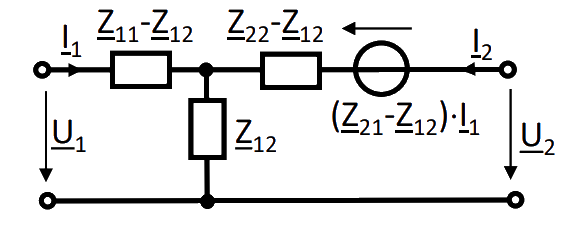
\includegraphics[width=0.7\columnwidth]{Zweipole/esb_t-mit_cs}
        \raggedright
        
    \item \textbf{$\mathbf{\Pi}$-ESB} bei gegebener $[\underline{Y}]$-Matrix:
    
        $Y_{12} \neq Y_{21}$ mit gesteuerter Quelle.
        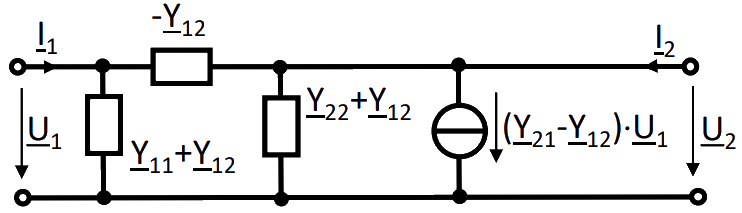
\includegraphics[width=0.8\columnwidth]{Zweipole/esb_pi-mit_cs}
        \raggedright
        
    \item  \textbf{Hybrid-ESB} bei gegebener [\underline{$H$}]-Matrix\\
    {\footnotesize Bsp.: ESB für NPN-Transistor.}
        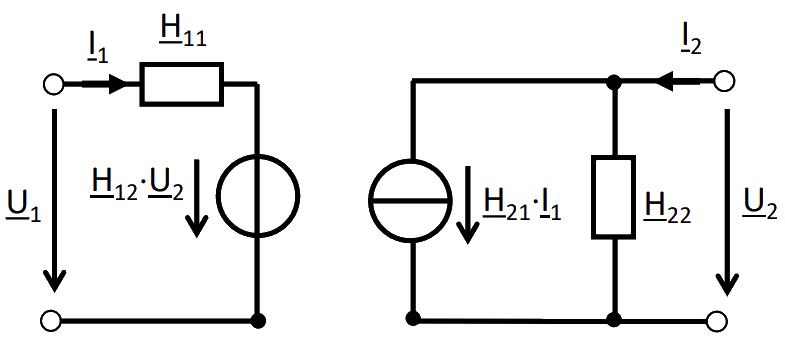
\includegraphics[width=0.7\columnwidth]{Zweipole/esb_hybrid-mit_cs}
\end{itemize}

\subsection{Beschaltete Zweitore}
\subsubsection{Ein- und Ausgangsimpedanz an Tor 1/2}
{\footnotesize $Z_V$: Last an Tor 2 $\rightarrow$ Eingangsimpedanz $Z_{e1}$, Betrieb von Seite 1\\ $Z_i$: Last an Tor 1 $\rightarrow$ Ausgangsimpedanz $Z_{e2}$, Betrieb von Seite 2}\\
\setlength{\parindent}{0pt}
\begin{minipage}{0.5\columnwidth}
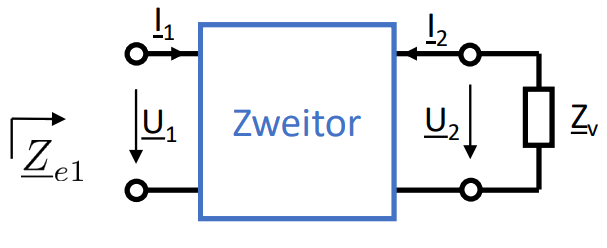
\includegraphics[width=\columnwidth]{Zweipole/Eingangsimpedanz}
\end{minipage}
\begin{minipage}{0.5\columnwidth}
	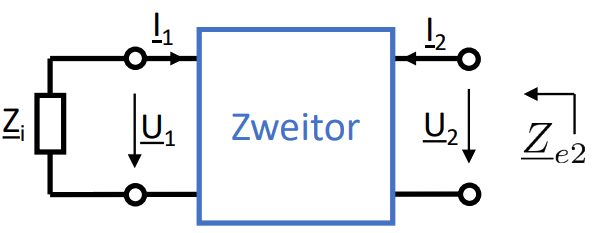
\includegraphics[width=\columnwidth]{Zweipole/Ausgangsimpedanz}
\end{minipage}
	\renewcommand{\arraystretch}{1.8}
	\arraycolsep=1.4pt
\begin{tabular}{|c|l|l|}

	\hline  & Last an Tor 2 & Last an Tor 1 \\
	\hline$Z$ & $ \underline{Z}_{e1} =  \underline{Z}_{11}-\frac{\underline{Z}_{12} \underline{Z}_{21}}{\underline{Z}_{22}+\underline{Z}_{V}}$ & $\underline{Z}_{e 2}=\underline{Z}_{22}-\frac{\underline{Z}_{12} \underline{Z}_{21}}{\underline{Z}_{11}+\underline{Z}_{i}}$ \\
	\hline
	$Y$ & $\underline{Y}_{e 1}=\underline{Y}_{11}-\frac{\underline{Y}_{12} \underline{Y}_{21}}{\underline{Y}_{22}+\underline{Y}_{V}}$ & $\underline{Y}_{e 2}=\underline{Y}_{22}-\frac{\underline{Y}_{12} \underline{Y}_{21}}{\underline{Y}_{11}+\underline{Y}_{i}}$ \\
	\hline
	$A$ & $\underline{Z}_{e 1}=\frac{A_{11} \underline{Z}_{v}+\underline{A}_{12}}{\underline{A}_{21} \underline{Z}_{v}+\underline{A}_{22}}$ & $\underline{Z}_{e 2}=\frac{\underline{A}_{22} \underline{Z}_{i}+\underline{A}_{12}}{\underline{Z}_{21} \underline{Z}_{i}+\underline{A}_{11}}$ \\
	\hline
	$H$ & $\underline{Z}_{e 1}=\underline{H}_{11}-\frac{\underline{H}_{12} \underline{H}_{21}}{\underline{H}_{22}+\underline{Y}_{V}}$ & $\underline{Y}_{e 2}=\underline{H}_{22}-\frac{\underline{H}_{12} \underline{H}_{21}}{\underline{H}_{11}+\underline{Z}_{i}}$ \\
	\hline
	$C$ & $\underline{Y}_{e1}=\underline{C}_{11}-\frac{C_{12} \underline{C}_{21}}{\underline{C}_{22}+\underline{Y}_{V}}$ & $\underline{Z}_{e 2}=\underline{C}_{22}-\frac{\underline{C}_{12} \underline{C}_{21}}{\underline{C}_{11}+\underline{Y}_{i}}$ \\
	\hline
\end{tabular}

%    \begin{flalign*}
%        \boldsymbol{Z}\rightarrow&\  \underline{Z}_{e1} = \underline{Z}_{11}-\frac{\underline{Z}_{12}\underline{Z}_{21}}{\underline{Z}_{22}+\underline{Z}_V}\\
%        \boldsymbol{Y}\rightarrow&\  \underline{Y}_{e1} = \underline{Y}_{11}-\frac{\underline{Y}_{12}\underline{Y}_{21}}{\underline{Y}_{22}+\underline{Y}_V}\\
%        \boldsymbol{A}\rightarrow&\  \underline{Z}_{e1} = \frac{\underline{A}_{11}\underline{Z}_V + \underline{A}_{12}}{\underline{A}_{21}\underline{Z}_V+\underline{A}_{22}}\\
%        \boldsymbol{H}\rightarrow&\  \underline{Z}_{e1} = \underline{H}_{11}-\frac{\underline{H}_{12}\underline{H}_{21}}{\underline{H}_{22}+\underline{Y}_V}\\
%        \boldsymbol{C}\rightarrow&\  \underline{Y}_{e1} = \underline{C}_{11}-\frac{\underline{C}_{12}\underline{C}_{21}}{\underline{C}_{22}+\underline{Z}_V}\\
%    \end{flalign*}
%\raggedright
%
%\subsubsection{Ausgangsimpedanz}
%\centering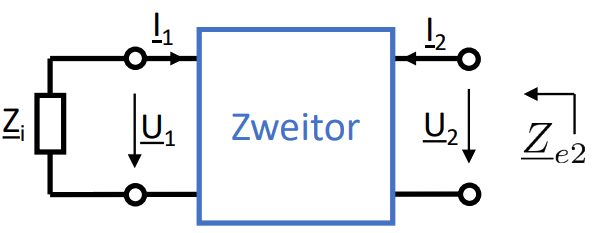
\includegraphics[width=0.5\columnwidth]{Zweipole/Ausgangsimpedanz}
%\begin{mdframed}[style=exercise]
%    \begin{align*}
%        \boldsymbol{Z}\rightarrow&\  \underline{Z}_{e2} = \underline{Z}_{22}-\frac{\underline{Z}_{12}\underline{Z}_{21}}{\underline{Z}_{11}+\underline{Z}_i}\\
%        \boldsymbol{Y}\rightarrow&\  \underline{Y}_{e2} = \underline{Y}_{22}-\frac{\underline{Y}_{12}\underline{Y}_{21}}{\underline{Y}_{11}+\underline{Y}_i}\\
%        \boldsymbol{A}\rightarrow&\  \underline{Z}_{e2} = \frac{\underline{A}_{22}\underline{Z}_i + \underline{A}_{12}}{\underline{A}_{21}\underline{Z}_i+\underline{A}_{11}}\\
%        \boldsymbol{H}\rightarrow&\  \underline{Z}_{e2} = \underline{H}_{22}-\frac{\underline{H}_{12}\underline{H}_{21}}{\underline{H}_{11}+\underline{Y}_i}\\
%        \boldsymbol{C}\rightarrow&\  \underline{Y}_{e2} = \underline{C}_{22}-\frac{\underline{C}_{12}\underline{C}_{21}}{\underline{C}_{11}+\underline{Z}_i}\\
%    \end{align*}
%\end{mdframed}
%\raggedright

\subsubsection{Ersatzquelle}
Berechnung Innenwiderstand $\underline{Z}_i$ eines Ersatz-Zweipols:\\ 
Quellen $U_q$ kurzschließen. $I_q$ unterbrechen.\\
Gilt nicht bei gesteuerten Quellen.\\
\begin{center}
	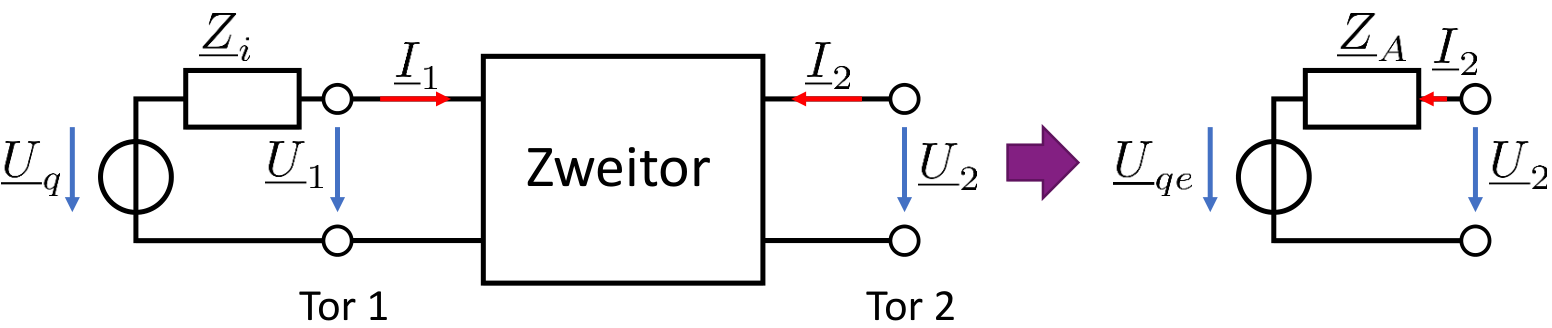
\includegraphics[width=\columnwidth]{Zweipole/Ersatzquelle_2}
\end{center}
\begin{tabularx}{\columnwidth}{|c|X|X|}
	\hline
	 & Quelle an Tor 1 & Quelle an Tor 2 \\
	\hline A & $\underline{U}_{q e}=\frac{1}{\underline{A}_{21} \underline{Z}_i+\underline{A}_{11}} \underline{U}_q$ & $\underline{U}_{q e}=\frac{\operatorname{det}(\underline{A})}{\underline{A}_{21} \underline{Z}_i+\underline{A}_{22}} \underline{U}_q$ \\
	\hline Z & $\underline{U}_{q e}=\frac{\underline{Z}_{21}}{\underline{Z}_{11}+\underline{Z}_i} \underline{U}_q$ & $\underline{U}_{q e}=\frac{\underline{Z}_{12}}{\underline{Z}_{22}+\underline{Z}_i} \underline{U}_q$ \\
	\hline Y & $\underline{I}_{q e}=-\frac{\underline{Y}_{21}}{\underline{Y}_{11}+\underline{Y}_i} \underline{I}_q$ & $\underline{I}_{q e}=-\frac{\underline{Y}_{12}}{\underline{Y}_{22}+\underline{Y}_i} \underline{I}_q$ \\
	\hline H & $\underline{I}_{q e}=-\frac{\underline{H}_{21}}{\underline{H}_{11}+\underline{Z}_i} \underline{U}_q$ & $\underline{U}_{q e}=\frac{\underline{H}_{12}}{\underline{H}_{22}+\underline{Y}_i} \underline{I}_q$ \\
	\hline
\end{tabularx}
\begin{tabularx}{\columnwidth}{|c|X|X|}
	\hline
	        & Quelle an Tor 1 & Quelle an Tor 2 \\
	\hline
	A & $Z_A = \frac{A_{22}Z_i + A_{12}}{A_{21}Z_i + A_{11}}$ & $Z_A = \frac{A_{11}Z_i + A_{12}}{A_{21}Z_i + A_{22}}$ \\
	\hline
	Z & $Z_A = Z_{22} - \frac{Z_{12} Z_{21}}{Z_{11} + Z_i}$ & $Z_A = Z_{11} - \frac{Z_{12} Z_{21}}{Z_{22} + Z_i}$ \\
	\hline
	Y & $Y_A = Y_{22} - \frac{Y_{12} Y_{21}}{Y_{11} + Y_i}$ & $Y_A = Y_{11} - \frac{Y_{12} Y_{21}}{Y_{22} + Y_i}$ \\
	\hline
	H & $Y_A = H_{22} - \frac{H_{12} H_{21}}{H_{11} + Z_i}$ & $Z_A = H_{11} - \frac{H_{12} H_{21}}{H_{22} + Y_i}$ \\
	\hline
\end{tabularx}
siehe Ausgangsimpedanz $Z_{e2} = Z_A$ (Quelle an Tor 1).

\subsubsection{Wellenwiderstand}
\begin{minipage}{0.5\columnwidth}
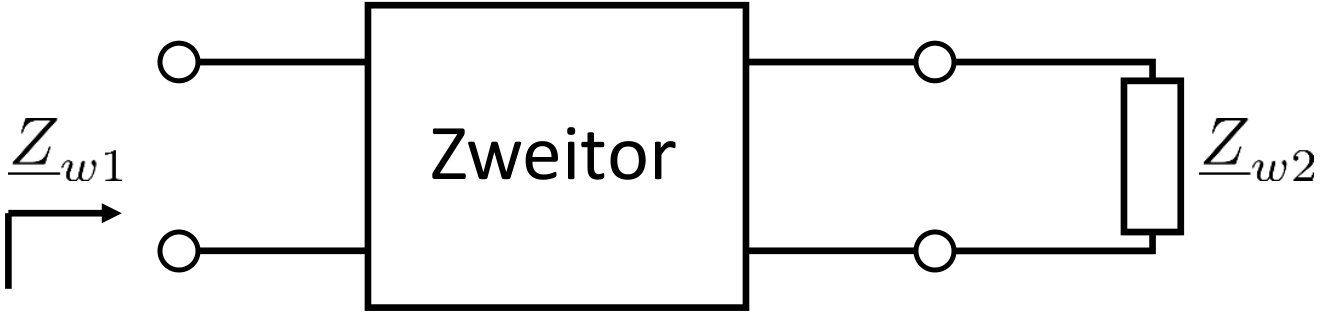
\includegraphics[width=\columnwidth]{Zweipole/wellenwiderstand_an_tor_2}
\end{minipage}
\begin{minipage}{0.5\columnwidth}
	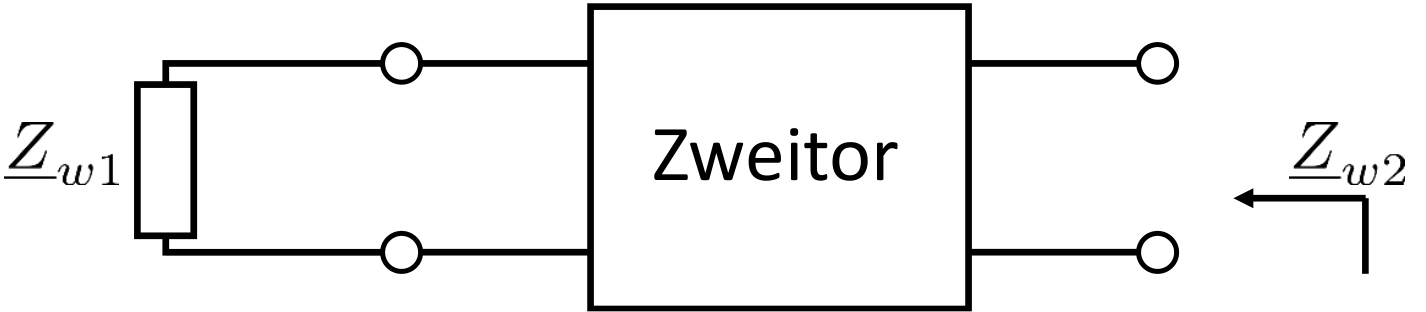
\includegraphics[width=\columnwidth]{Zweipole/wellenwiderstand_an_tor_1}
\end{minipage}
\begin{gather*}
	\boxed{
	\underline{Z}_{w1} = \frac{\underline{A}_{11}\underline{Z}_{w2} + \underline{A}_{12}}{\underline{A}_{21}\underline{Z}_{w2}+\underline{A}_{22}}
	} \qquad \boxed{
  	\underline{Z}_{w2} = \frac{\underline{A}_{22}\underline{Z}_{w1} + \underline{A}_{12}}{\underline{A}_{21}\underline{Z}_{w1}+\underline{A}_{11}}
  	}
\end{gather*}
\begin{minipage}{0.5\columnwidth}
\renewcommand{\arraystretch}{2}
	symmetrische ZT: $\underline{Z}_{w1}=\underline{Z}_{w2}$\\
	\begin{tabular}{|c|c|c|}
		\hline
		& $\boldsymbol{\underline{Z}_{w1}}$ & $\boldsymbol{\underline{Z}_{w2}}$
		\\
		\hline
		$\underline{\boldsymbol{Z}}$ & $\sqrt{\frac{\underline{Z}_{11}\operatorname{det}\underline{Z}}{\underline{Z}_{22}}}$ & $\sqrt{\frac{\underline{Z}_{22}\operatorname{det}\underline{Z}}{\underline{Z}_{11}}}$
		\\
		\hline
		$\underline{\boldsymbol{Y}}$ & $\sqrt{\frac{\underline{Y}_{22}}{\underline{Y}_{11}\operatorname{det}\underline{Y}}}$ & $\sqrt{\frac{\underline{Y}_{11}}{\underline{Y}_{22}\operatorname{det}\underline{Y}}}$
		\\
		\hline
		$\underline{\boldsymbol{A}}$ & $\sqrt{\frac{\underline{A}_{11}\cdot\underline{A}_{12}}{\underline{A}_{21}\cdot\underline{A}_{22}}}$ & $\sqrt{\frac{\underline{A}_{22}\cdot\underline{A}_{12}}{\underline{A}_{21}\cdot\underline{A}_{11}}}$
		\\
		\hline
		$\underline{\boldsymbol{H}}$ & $\sqrt{\frac{\underline{H}_{11}\operatorname{det}\underline{H}}{\underline{H}_{22}}}$ & $\sqrt{\frac{\underline{H}_{11}}{\underline{H}_{22}\operatorname{det}\underline{H}}}$
		\\
		\hline
		$\underline{\boldsymbol{C}}$ & $\sqrt{\frac{\underline{C}_{22}}{\underline{C}_{11}\operatorname{det}\underline{C}}}$ & $\sqrt{\frac{\underline{C}_{11}\operatorname{det}\underline{C}}{\underline{C}_{11}}}$
		\\
		\hline
	\end{tabular}
\end{minipage}
\begin{minipage}{0.5\columnwidth}
	\small
	\begin{itemize}
	\item[] Messtechnische\\ Ermittlung:
	
	$Z_{01}$: Leerlauf - Tor 1\\
	$Z_{k1}$: Kurzschluss - Tor 1
	\end{itemize}
	\begin{align*}
		\underline{Z}_{w1} &= \sqrt{\underline{Z}_{k1}\cdot\underline{Z}_{01}}\\
		&=\sqrt{\frac{\underline{A}_{11}\cdot\underline{A}_{12}}{\underline{A}_{21}\cdot\underline{A}_{22}}}\\
		\underline{Z}_{w2} &= \sqrt{\underline{Z}_{k2}\cdot\underline{Z}_{02}}\\
		&=\sqrt{\frac{\underline{A}_{22}\cdot\underline{A}_{12}}{\underline{A}_{21}\cdot\underline{A}_{11}}}
	\end{align*}
\end{minipage}

    
\subsubsection{Scheinleistungsanpassung}
\begin{minipage}{0.55\columnwidth}
	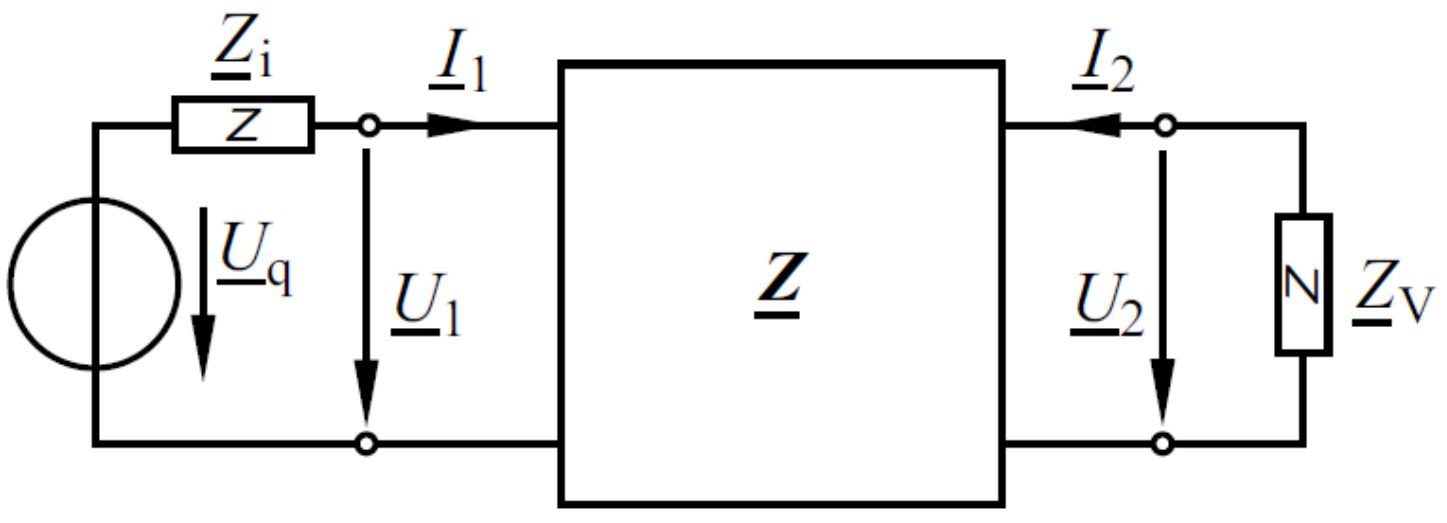
\includegraphics[width=\columnwidth]{Zweipole/scheinleistungsanpassung}
\end{minipage}
\begin{minipage}{0.45\columnwidth}
$\quad \underline{Z}_i = \underline{Z}_{w1} \quad \underline{Z}_V=\underline{Z}_{w2}
$
\end{minipage}

Beschaltet man jedes Tor mit seinem Wellenwiderstand, so liegt Scheinleistungsanpassung vor.

\subsubsection{Kettenwiderstand}
\begin{minipage}{0.5\columnwidth}
	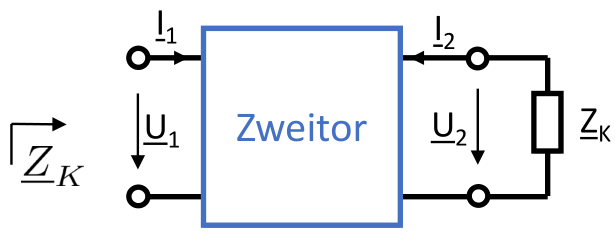
\includegraphics[width=\columnwidth]{Zweipole/Kettenwiderstand}
\end{minipage}
\begin{minipage}[b]{0.5\columnwidth}
	$$
	\underline{Z}_K = \underline{Z}_{11} - \frac{\underline{Z}_{12}\underline{Z}_{21}}{\underline{Z}_{22}+\underline{Z}_K}
	$$
\end{minipage}
\\
\small
Schaltet man eine große Zahl gleicher ZT in Kette, so nähert sich der Eingangswiderstand dem Kettenwiderstand $\mathbf{\underline{Z}_K}$ an.\\
L\"osung der obigen Gleichung:
\[
    \underline{Z}_K = \frac{1}{2}(\underline{Z}_{11} - \underline{Z}_{22} \pm \sqrt{(\underline{Z}_{11}-\underline{Z}_{22})^2+4\cdot\operatorname{det}\underline{Z}})
\]
Symmetrische ZT: Kettenwiderstand = Wellenwiderstand.
\normalsize
